\documentclass[10pt,a4paper]{article}
\usepackage[a4paper,margin=1.9cm]{geometry}
\usepackage[T1]{fontenc}
\usepackage{mathptmx}
\usepackage{microtype}
\usepackage{amsmath}
\usepackage{graphicx}
\usepackage{booktabs}
\usepackage{multirow}
\usepackage[font=small,labelfont=bf,skip=3pt]{caption}
\usepackage{enumitem}
\usepackage{titlesec}
\usepackage{xcolor}
\usepackage[colorlinks=true,linkcolor=blue!50!black,citecolor=blue!50!black,urlcolor=blue!50!black]{hyperref}

\titlespacing*{\section}{0pt}{6pt}{2pt}
\titleformat*{\section}{\large\bfseries}
\setlength{\parskip}{2pt}
\setlist{nosep,leftmargin=*}
\graphicspath{{../results/figures/}}

% every number below comes from ../results/tables/macros.tex (generated from the run logs)
\makeatletter
\@namedef{r@lora-lm-2e-4-acc150}{54.1}
\@namedef{r@lora-lm-2e-4-acc300}{55.7}
\@namedef{r@lora-lm-2e-4-acc50}{51.8}
\@namedef{r@lora-lm-2e-4-gnorm}{1.9}
\@namedef{r@lora-lm-2e-4-loss}{0.687}
\@namedef{r@lora-lm-2e-4-s2t}{25/25}
\@namedef{r@lora-lm-2e-4-train}{0.72}
\@namedef{r@lora-lm-2e-5-acc150}{51.1}
\@namedef{r@lora-lm-2e-5-acc300}{51.3}
\@namedef{r@lora-lm-2e-5-acc50}{48.2}
\@namedef{r@lora-lm-2e-5-gnorm}{6.6}
\@namedef{r@lora-lm-2e-5-loss}{0.948}
\@namedef{r@lora-lm-2e-5-s2t}{200/150}
\@namedef{r@lora-lm-2e-5-train}{1.10}
\@namedef{r@pissa-lm-2e-4-acc150}{51.9}
\@namedef{r@pissa-lm-2e-4-acc300}{56.1}
\@namedef{r@pissa-lm-2e-4-acc50}{52.2}
\@namedef{r@pissa-lm-2e-4-gnorm}{9.4}
\@namedef{r@pissa-lm-2e-4-loss}{0.688}
\@namedef{r@pissa-lm-2e-4-s2t}{25/10}
\@namedef{r@pissa-lm-2e-4-train}{0.51}
\@namedef{r@pissa-lm-2e-5-acc150}{53.2}
\@namedef{r@pissa-lm-2e-5-acc300}{54.6}
\@namedef{r@pissa-lm-2e-5-acc50}{51.9}
\@namedef{r@pissa-lm-2e-5-gnorm}{18.1}
\@namedef{r@pissa-lm-2e-5-loss}{0.717}
\@namedef{r@pissa-lm-2e-5-s2t}{25/25}
\@namedef{r@pissa-lm-2e-5-train}{0.75}
\@namedef{r@pl-cross-150-diff}{$-0.9$}
\@namedef{r@pl-cross-150-hi}{$+0.8$}
\@namedef{r@pl-cross-150-lo}{$-2.5$}
\@namedef{r@pl-cross-150-p}{0.320}
\@namedef{r@pl-cross-300-diff}{$-1.1$}
\@namedef{r@pl-cross-300-hi}{$+0.6$}
\@namedef{r@pl-cross-300-lo}{$-2.9$}
\@namedef{r@pl-cross-300-p}{0.194}
\@namedef{r@pl-cross-50-diff}{$+0.1$}
\@namedef{r@pl-cross-50-hi}{$+1.8$}
\@namedef{r@pl-cross-50-lo}{$-1.5$}
\@namedef{r@pl-cross-50-p}{0.909}
\@namedef{r@pl-high-150-diff}{$-2.2$}
\@namedef{r@pl-high-150-hi}{$+0.3$}
\@namedef{r@pl-high-150-lo}{$-4.7$}
\@namedef{r@pl-high-150-p}{0.091}
\@namedef{r@pl-high-300-diff}{$+0.4$}
\@namedef{r@pl-high-300-hi}{$+2.8$}
\@namedef{r@pl-high-300-lo}{$-2.1$}
\@namedef{r@pl-high-300-p}{0.774}
\@namedef{r@pl-high-50-diff}{$+0.4$}
\@namedef{r@pl-high-50-hi}{$+3.0$}
\@namedef{r@pl-high-50-lo}{$-2.1$}
\@namedef{r@pl-high-50-p}{0.763}
\@namedef{r@pl-low-150-diff}{$+2.2$}
\@namedef{r@pl-low-150-hi}{$+5.1$}
\@namedef{r@pl-low-150-lo}{$-0.7$}
\@namedef{r@pl-low-150-p}{0.137}
\@namedef{r@pl-low-300-diff}{$+3.3$}
\@namedef{r@pl-low-300-hi}{$+6.2$}
\@namedef{r@pl-low-300-lo}{$+0.5$}
\@namedef{r@pl-low-300-p}{0.020}
\@namedef{r@pl-low-50-diff}{$+3.7$}
\@namedef{r@pl-low-50-hi}{$+6.9$}
\@namedef{r@pl-low-50-lo}{$+0.4$}
\@namedef{r@pl-low-50-p}{0.025}
\@namedef{r@spec-connector-effrank}{91}
\@namedef{r@spec-connector-energy}{6.9}
\@namedef{r@spec-connector-minor}{1.15}
\@namedef{r@spec-connector-scale}{7.0}
\@namedef{r@spec-lm-effrank}{62}
\@namedef{r@spec-lm-energy}{18.5}
\@namedef{r@spec-lm-minor}{0.36}
\@namedef{r@spec-lm-scale}{10.5}
\@namedef{r@spec-vision-effrank}{56}
\@namedef{r@spec-vision-energy}{13.1}
\@namedef{r@spec-vision-minor}{0.09}
\@namedef{r@spec-vision-scale}{4.3}
\@namedef{r@zs-acc}{49.6}
\@namedef{r@zs-loss}{8.06}
\makeatother
\makeatletter
\@namedef{r@spec-lm-s1min}{6.0}
\@namedef{r@spec-vision-s1min}{1.4}
\@namedef{r@spec-lm-s1max}{18.5}
\@namedef{r@spec-vision-s1max}{4.9}
\makeatother

\newcommand{\R}[1]{\ifcsname r@#1\endcsname\csname r@#1\endcsname\else\textbf{??}\fi}

\title{\vspace{-1.4cm}\Large\textbf{Does PiSSA's faster convergence transfer to a small vision--language model?}}
\author{Imanchana Kaveeshwara Bandara (220059J) \\ \small EN4554 Deep Learning for Vision, Assignment 1, Part 1 \\
\small Code: \url{https://github.com/KaveeshwaraBandara/en4554-lora-vlm-tool-agent}}
\date{\vspace{-0.9cm}}

\begin{document}
\maketitle

\section{Central claim of the paper}
PiSSA~\cite{pissa} keeps LoRA's form $W = W^{\text{res}} + BA$~\cite{lora} but initialises $A=\sqrt{S_{[:r]}}\,V^\top_{[:r]}$ and $B=U_{[:r]}\sqrt{S_{[:r]}}$ from the top-$r$ singular triplets of the pretrained weight, freezing the residual $W^{\text{res}}$. Because the adapter starts in the principal subspace, PiSSA claims to \emph{converge faster and reach better performance than LoRA with the same number of trainable parameters} (e.g.\ Mistral-7B on GSM8K: 72.86\% vs.\ 67.7\%).

\section{Concept chosen and the evidence for it}
We test the \textbf{faster-convergence} claim. In the paper's Sec.~5.2 / Fig.~4 (LLaMA~2-7B on MetaMathQA-395K), PiSSA's training loss falls faster in the first $\sim$100 steps and stays below LoRA's, its gradient norm is much larger than LoRA's and follows the trend of full fine-tuning, and GSM8K accuracy is higher throughout. The paper attributes LoRA's slow start to its initialisation ($A$ Gaussian, $B=0$), which makes early gradients small. Its App.~A ablation (principal $>$ medium $>$ minor singular components) supports the subspace explanation.

\section{Translated hypotheses}
\begin{itemize}
\item[\textbf{H1}] When SmolVLM-256M is fine-tuned on a text-reading VQA task with equal-rank adapters and the paper's hyper-parameters, PiSSA lowers the held-out answer loss in fewer steps than LoRA, with larger gradient norms, and gives higher accuracy at fixed step budgets.
\item[\textbf{H1$'$}] (control) The advantage remains when LoRA uses its usual $10\times$ larger learning rate, i.e.\ it is not merely a larger effective step size.
\item[\textbf{H2}] (vision-specific) PiSSA's head start depends on how much of each weight matrix its top-$r$ directions hold. If the SigLIP vision encoder has flatter spectra than the language model, PiSSA's edge should shrink when the vision tower is adapted.
\end{itemize}

\section{Experimental setup}
\textbf{Model.} SmolVLM-256M-Instruct~\cite{smolvlm}: SigLIP-B/16-512 vision encoder~\cite{siglip}, pixel-shuffle connector, SmolLM2-135M; 256M parameters ($\le$500M).
\textbf{Data.} TextVQA~\cite{textvqa} \emph{validation} split, streamed with a fixed seed: 2{,}000 training and 500 evaluation questions, disjoint by image. We use the validation split because SmolVLM's training mix (The Cauldron) contains the TextVQA train split, so these questions are unseen. TextVQA was chosen by a zero-shot headroom check on 200 questions per dataset (TextVQA 51.0, DocVQA 48.4 ANLS, OK-VQA 35.1, VQAv2 70.9). OK-VQA has more headroom, but its gap is world knowledge a 135M language model cannot learn from 2k examples, and it barely depends on the vision tower, which H2 needs. Images are resized to a 1024-px longest edge (4 tiles + global view, 320 image tokens): the same zero-shot accuracy as the default 2048~px (51.0 vs.\ 51.1) at $2.7\times$ shorter sequences.
\textbf{Adapters.} All 7 projections of the 30 language-model layers (210 matrices), $r=16$, $\alpha=r$, dropout 0 as in the paper; 4.88M trainable parameters (1.9\%). PiSSA uses PEFT's \texttt{init\_lora\_weights="pissa"}; our own SVD initialisation (used for the minor-component ablation) reproduces it exactly (unit test).
\textbf{Training.} AdamW without weight decay, cosine schedule with 3\% warm-up, batch 8, 300 steps ($\approx$1.2 epochs), gradient clipping 1.0, loss on the answer tokens only (majority answer as target). Learning rates $2\!\times\!10^{-5}$ (the paper's) and $2\!\times\!10^{-4}$ (typical for LoRA). fp32 master weights with fp16 autocast (the T4 has no bf16; initial loss scale $2^{12}$, no skipped steps). Seeds 42 and 43; with the same seed both methods see identical batches.
\textbf{Metrics tied to the claim.} Held-out answer NLL on 256 eval questions at steps 0, 5, 10, 25, 50, 100, \dots, 300 and the number of steps to reach NLL $\le 1$; training loss; pre-clip gradient norm; VQA accuracy~\cite{vqa} (10 annotators) on the 500 eval questions after 50, 150 and 300 steps, with paired bootstrap 95\% CIs over questions (seeds averaged).
\textbf{Deviations from the paper:} batch 8 (not 128), fp16 autocast (not fp32), 300 steps.

\section{Results and interpretation}
\begin{table}[h]
\centering\small
\caption{Language-model adapters on TextVQA (mean of 2 seeds, $\pm$ half the seed range). Accuracy in \%, held-out loss = answer NLL after 300 steps; steps to loss $\le$1 per seed (loss evaluated at steps 0, 5, 10, 25, 50, 100, \dots); train loss = mean of the last 50 steps.}
\label{tab:main}
\begin{tabular}{llcccccc}
\toprule
Method & lr & acc@50 & acc@150 & acc@300 & held-out loss & steps to loss$\le$1 & train loss \\
\midrule
Zero-shot & -- & \multicolumn{3}{c}{49.6} & 8.06 & -- & -- \\
LoRA & 2e-5 & 48.2\,$\pm$0.1 & 51.1\,$\pm$0.1 & 51.3\,$\pm$0.1 & 0.948 & 200/150 & 1.10 \\
\textbf{PiSSA} & \textbf{2e-5} & \textbf{51.9\,$\pm$0.5} & \textbf{53.2\,$\pm$0.3} & \textbf{54.6\,$\pm$0.4} & \textbf{0.717} & \textbf{25/25} & \textbf{0.75} \\
LoRA & 2e-4 & 51.8\,$\pm$0.1 & 54.1\,$\pm$0.5 & 55.7\,$\pm$0.1 & 0.687 & 25/25 & 0.72 \\
PiSSA & 2e-4 & 52.2\,$\pm$1.1 & 51.9\,$\pm$0.7 & 56.1\,$\pm$0.5 & 0.688 & 25/10 & 0.51 \\
\bottomrule
\end{tabular}

\end{table}
\vspace{-6pt}
\begin{figure}[h]
\centering
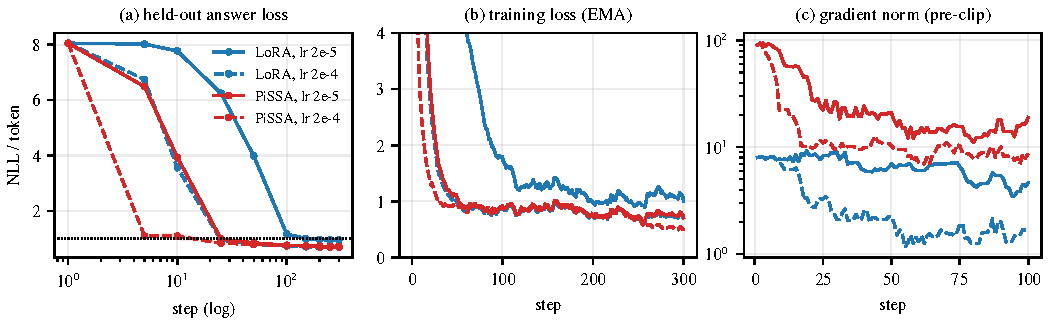
\includegraphics[width=\linewidth]{fig_convergence.pdf}
\caption{Convergence metrics tied to the claim (mean of seeds; band = seed range in (a); step 0 drawn at 1 on the log axis; dotted line = loss 1). Blue = LoRA, red = PiSSA; solid = lr $2\!\times\!10^{-5}$, dashed = $2\!\times\!10^{-4}$.}
\label{fig:conv}
\end{figure}

\textbf{An answer-format phase.} At step 0 the held-out NLL is \R{zs-loss} although zero-shot accuracy is \R{zs-acc}\%: SmolVLM answers in sentence case with a full stop (``Chamberlain.''), whereas TextVQA references are lowercase. The first training steps mostly teach this format, so the steps needed to reach NLL $\le$1 measure how quickly the model adapts. Accuracy, whose normalisation ignores case and punctuation, measures the content.

\textbf{H1 is supported at the paper's learning rate.} At $2\!\times\!10^{-5}$, PiSSA reaches NLL $\le$1 at step \R{pissa-lm-2e-5-s2t} (seeds 42/43) vs.\ \R{lora-lm-2e-5-s2t} for LoRA (Fig.~\ref{fig:conv}a). Its median gradient norm over steps 10--100 is \R{pissa-lm-2e-5-gnorm} vs.\ \R{lora-lm-2e-5-gnorm} (Fig.~\ref{fig:conv}c), the pattern of the paper's Fig.~4. It is more accurate at all three budgets, significantly so after 50 and 300 steps (\R{pl-low-300-diff} points [\R{pl-low-300-lo}, \R{pl-low-300-hi}], $p=\R{pl-low-300-p}$; Table~\ref{tab:paired}), and its held-out loss stays lower (\R{pissa-lm-2e-5-loss} vs.\ \R{lora-lm-2e-5-loss}). Both seeds agree.

\textbf{H1$'$ is not supported.} At $2\!\times\!10^{-4}$, LoRA converges as quickly (NLL $\le$1 at step \R{lora-lm-2e-4-s2t}) and ends at the same held-out loss (\R{lora-lm-2e-4-loss} vs.\ \R{pissa-lm-2e-4-loss}) and accuracy (\R{pl-high-300-diff} [\R{pl-high-300-lo}, \R{pl-high-300-hi}]). PiSSA's \emph{training} loss is still lower (\R{pissa-lm-2e-4-train} vs.\ \R{lora-lm-2e-4-train}), so it fits the training set faster without generalising better. Its accuracy after 150 steps is lower in both seeds (\R{pissa-lm-2e-4-acc150} vs.\ \R{lora-lm-2e-4-acc150}; \R{pl-high-150-diff} [\R{pl-high-150-lo}, \R{pl-high-150-hi}]), which hints at instability but is not significant. Most tellingly, PiSSA at the paper's learning rate and LoRA at a $10\times$ larger one have almost identical loss curves (red solid vs.\ blue dashed in Fig.~\ref{fig:conv}a,b), and their accuracies are statistically indistinguishable at every budget (\R{pl-cross-300-diff} [\R{pl-cross-300-lo}, \R{pl-cross-300-hi}] after 300 steps).

\textbf{Why: the spectrum sets the effective step.} Under Adam each step changes $W$ by $\approx \Delta B\,A + B\,\Delta A$. LoRA starts with $B=0$ and $\|A\|_F=\sqrt{r/3}$ (PEFT's Kaiming init; we measured 0.577 per row), whereas PiSSA starts with $\|A\|_F=\|B\|_F=(\sum_{i\le r}\sigma_i)^{1/2}$. On SmolLM2's 210 matrices the ratio $(\|A\|_F{+}\|B\|_F)^{\text{PiSSA}}/\|A\|_F^{\text{LoRA}}$ averages \R{spec-lm-scale}$\times$ and is nearly constant with depth (Fig.~\ref{fig:vision}b), which matches the $10\times$ learning-rate gap that equalises the two methods. In this setting, PiSSA's faster convergence acts as a learning-rate amplifier set by the singular values.

\begin{table}[h]
\centering\small
\caption{Paired accuracy differences (points) on the same 500 questions, seeds averaged; bootstrap 95\% CI; $^{*}$ CI excludes 0.}
\label{tab:paired}
\begin{tabular}{lccc}
\toprule
Accuracy difference (points) & step 50 & step 150 & step 300 \\
\midrule
PiSSA $-$ LoRA, lr 2e-5 & $+3.7$ [$+0.4$, $+6.9$]$^{*}$ & $+2.2$ [$-0.7$, $+5.1$] & $+3.3$ [$+0.5$, $+6.2$]$^{*}$ \\
PiSSA $-$ LoRA, lr 2e-4 & $+0.4$ [$-2.1$, $+3.0$] & $-2.2$ [$-4.7$, $+0.3$] & $+0.4$ [$-2.1$, $+2.8$] \\
PiSSA 2e-5 $-$ LoRA 2e-4 & $+0.1$ [$-1.5$, $+1.8$] & $-0.9$ [$-2.5$, $+0.8$] & $-1.1$ [$-2.9$, $+0.6$] \\
\bottomrule
\end{tabular}

\end{table}
\vspace{-6pt}
\begin{figure}[h]
\centering
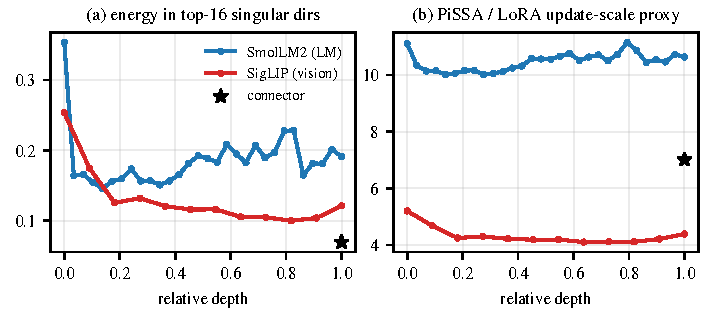
\includegraphics[width=0.72\linewidth]{fig_vision.pdf}
\caption{Spectra of the matrices PiSSA initialises from, by relative depth (star = connector). (a) Share of each matrix's energy held by its top-16 singular directions. (b) PiSSA/LoRA update-scale proxy.}
\label{fig:vision}
\end{figure}

\textbf{H2: the vision tower is different.} SigLIP's matrices have much smaller singular values than SmolLM2's (the mean $\sigma_1$ per matrix type is \R{spec-vision-s1min}--\R{spec-vision-s1max} vs.\ \R{spec-lm-s1min}--\R{spec-lm-s1max}) and flatter spectra: their top-16 directions hold \R{spec-vision-energy}\% of the energy vs.\ \R{spec-lm-energy}\% (Fig.~\ref{fig:vision}a). The pixel-shuffle connector is the flattest (\R{spec-connector-energy}\%). PiSSA's update-scale proxy is therefore only \R{spec-vision-scale}$\times$ in the vision tower vs.\ \R{spec-lm-scale}$\times$ in the language model. By the mechanism above, adapting the vision encoder with PiSSA should behave like LoRA with a $\sim$4$\times$ (not $\sim$10$\times$) larger learning rate. PiSSA's head start should be correspondingly smaller there, while a larger share of the pretrained visual function stays in the frozen residual. This is a vision-specific prediction the language-only paper cannot make.

\textbf{Conclusion.} On a small VLM, PiSSA's faster convergence transfers at the paper's hyper-parameters (H1), but the better-final-performance part does not once LoRA's learning rate is tuned (H1$'$). The head start is quantitatively explained by a larger effective step size set by the weight spectrum, which is $\sim$2.4$\times$ weaker in the SigLIP vision tower (H2). \emph{Limitations:} two seeds, 300 steps, batch 8, one model and task; the vision-tower prediction is derived from the spectra and was not confirmed by training runs within the free-tier GPU budget.

\vspace{-4pt}
{\footnotesize
\begin{thebibliography}{9}\setlength{\itemsep}{0pt}
\bibitem{pissa} F.~Meng, Z.~Wang, M.~Zhang. PiSSA: Principal singular values and singular vectors adaptation of large language models. \emph{NeurIPS}, 2024.
\bibitem{lora} E.~J.~Hu et al. LoRA: Low-rank adaptation of large language models. \emph{ICLR}, 2022.
\bibitem{smolvlm} A.~Marafioti et al. SmolVLM: Redefining small and efficient multimodal models. arXiv:2504.05299, 2025.
\bibitem{siglip} X.~Zhai, B.~Mustafa, A.~Kolesnikov, L.~Beyer. Sigmoid loss for language image pre-training. \emph{ICCV}, 2023.
\bibitem{textvqa} A.~Singh et al. Towards VQA models that can read. \emph{CVPR}, 2019.
\bibitem{vqa} S.~Antol et al. VQA: Visual question answering. \emph{ICCV}, 2015.
\end{thebibliography}}
\end{document}
